\chapter{The PyTCHInt Library}
\label{chap:pytchint}

This appendix is based on the following software, to be released:\\
\fullcite{tchint}

The basis for how the library works is partially discussed in the following paper and its supplementary material: \\
\fullcite{cohenSimilarity2019}

\section{Introduction}

All transcorrelated matrix element calculations presented in this dissertation have been performed using the group's \tchint library or its Python extension, \pytchint. This library works by either producing transformed integral files, dubbed \fcidump files for four-index integrals,\supercite{knowlesDeterminant1989} or \tcdump files for the \gls{TC} six-index integrals. Note that since the \gls{TC} transformation is non-Hermitian, we do not have the same symmetries in these files as we do with conventional methods, or by interfacing with another program (such as \neci) or the Python interpreter (in the case of \pytchint).

As described in section \ref{sec:tc},
\begin{equation}
\begin{split}
    \htc = &\sum_{pq}\sum_\sigma h_q^p a_{p\sigma}^\dagger a_{q\sigma}
    + \frac{1}{2} \sum_{pqrs} \big(V_{rs}^{pq} - K_{rs}^{pq}\big) \sum_{\sigma\tau}
    a_{p\sigma}^\dagger a_{q\tau}^\dagger a_{s\tau} a_{r\sigma} \\
    &- \frac{1}{6} \sum_{pqrstu} L_{stu}^{pqr}\sum_{\sigma\tau\lambda}
    a_{p\sigma}^\dagger a_{q\tau}^\dagger a_{r\lambda}^\dagger a_{u\lambda} a_{t\tau} a_{s\sigma},
\end{split}
\end{equation}
where
\begin{equation}
\begin{split}
    h_q^p &= \bra{p}h\ket{q}, \\
    V_{rs}^{pq} &= \bra{p q } r_{12}^{-1} \ket{ r s}, \\
    K_{rs}^{pq} &= \bra{p q } \hat{K} \ket{ r s}, \\
    L_{stu}^{pqr} &= \bra{p q r } \hat{L} \ket{s t u}.
\end{split}
\end{equation}
$h_q^p$ and $V_{rs}^{pq}$ are the one- and two-body terms from the electronic Schr\"odinger equation, familiar from conventional methods. Therefore, the key quantities to be evaluated by \tchint are the non-Hermitian two-body integrals $K_{rs}^{pq}$ and the Hermitian three-body integrals $L_{stu}^{pqr}$.

Once these integrals are evaluated, as long as we take care about using the correct bra and ket (a detail not important for Hermitian problems), many different methodologies can be applied with these integrals, such as the frozen-core approximation,\supercite{finkApproach1972,baerendsSelfconsistent1973,sachsFrozen1975} or \gls{xTC}.\supercite{christlmaierXTC2023}

\section{Matrix Element Evaluation}
The matrix elements not present in conventional methods are $K_{rs}^{pq}$ and $L_{stu}^{pqr}$. For these, we integrate on a grid, typically Treutler-Ahlrichs integration grids,
\supercite{beckeMulticenter1988,treutlerEfficient1995} which are atom-centred grids commonly used in density functional theory. These grids are obtained via \pyscf.

The two-electron matrix elements we need to evaluate are:
\begin{align}
    K_{rs}^{pq(1)} &= \bra{pq}\nabla_1u(\bm r_1, \bm r_2)\cdot\nabla_1\ket{rs}\\
    K_{rs}^{pq(2)} &= \bra{pq}\nabla_1^2u(\bm r_1, \bm r_2)\ket{rs}\\
    K_{rs}^{pq(3)} &= \bra{pq}(\nabla_1u(\bm r_1, \bm r_2))^2\ket{rs}.
\end{align}
Discretising on a grid of $N_\mathrm{grid}$ points with weights $w$, we have
\begin{equation}
    K_{rs}^{pq(1)} = \sum_{mn}^{N_\mathrm{grid}}
    \phi_p(\bm r_m)\nabla_{\bm r_m}\phi_r(\bm r_m)\cdot \nabla_{\bm r_m}u(\bm r_m, \bm r_n)\phi_q(\bm r_n)\phi_s(\bm r_n)w(\bm r_m)w(\bm r_n).
\end{equation}
Naive integration of this value yields $\mathcal{O}(N_\mathrm{grid}^2M^4)$ performance (where $M$ is the number of basis functions). However, we may improve this by first integrating over one coordinate and storing the intermediate value. Moreover, for $K_{rs}^{pq(2)}$, it is more efficient to integrate by parts. Therefore, for the full $K$ matrix, we calculate the intermediate value
\begin{align}
    X_s^q(\bm r_2) =& \int\d^3 r_1\ \nabla_1u(\bm r_1, \bm r_2)\cdot[\phi_p(\bm r_1) \nabla_1\phi_r(\bm r_1) - \phi_r(\bm r_1)
\nabla_1\phi_p(\bm r_1)]  \\
&+ \int\d^3 r_1\ \phi_p(\bm r_1)(\nabla u(\bm r_1, \bm r_2))^2 \phi_r(\bm r_1).
\end{align}
We can then obtain the $K$ matrix by
\begin{equation}
    K_{rs}^{pq} = \int\d^3 r_2\ \phi_q(\bm r_2)X_s^q(\bm r_2)\phi_s(\bm r_2)
\end{equation}
for a cost of $\mathcal{O}(N_\mathrm{grid}^2M^2+N_\mathrm{grid}M^4)$.

The three-body matrix,
\begin{equation}
    L^{pqr}_{stu} = \bra{pqr}\nabla_1u(\bm r_1, \bm r_2)\cdot \nabla u_1(\bm r_1, \bm r_3)\ket{stu}
\end{equation}
may similarly be resolved by calculating the intermediate value
\begin{equation}
    \bm Y_{qt}(\bm r_1) = \int\d^3 r_2\ \phi_q(\bm r_2)\nabla_1u(\bm r_1, \bm r_2)\phi_t(\bm r_2)
\end{equation}
to give
\begin{equation}
    L^{pqr}_{stu} = \int\d^3 r_1\ \phi_p(\bm r_1)\bm Y_{qt}(\bm r_1)\cdot\bm Y_{ru}(\bm r_1)\phi_s(\bm r_1).
\end{equation}

These integrations are simply parallelisable, and \tchint takes advantage of this by leveraging distributed memory with the \gls{MPI}\supercite{mpi41,dalcinMPI2005,dalcinMPI2008,dalcinParallel2011} standard and the OpenMP\supercite{dagumOpenMP1998} \gls{API}. We also make liberal use of BLAS\supercite{blackford2002updated} routines for further performance gains. Moreover, we take advantage of the fact that $L$ is Hermitian, substantially reducing storage requirements. We may also store $L$ sparsely since many elements are small, or use the \gls{xTC} approximation to bypass storing $L$ altogether and instead calculating modified four-index integrals and outputting a non-Hermitian \fcidump.

\section{Interface}

\tchint is predominantly written in Fortran, but most of the important interfacing subroutines (such as returning given matrix elements) have C bindings. This allows \tchint to be easily interfaced with other libraries, notably for \gls{TC}-\gls{FCIQMC} in \neci\supercite{gutherNECI2020} and \mseven.\supercite{andersonRobertanderson2024} By using this interface, these programs may be used to perform transcorrelated calculations, with all the features present in \tchint.

\tchint has also been given a Python interface called \pytchint by making use of the Cython language extension.\supercite{behnel2008cython,behnel2011cython,smithCython2015} Cython features C-like performance with easy integration in Python to allow for interactive computing and interfacing with the vast scientific package ecosystem available in Python. Python is typically also easier for rapid prototyping, a crucial feature in the world of scientific research, while Cython provides efficiency and a comprehensive profiling toolset.

With \pytchint, a user might interactively work with transcorrelated integrals by first calculating them,
\begin{lstlisting}[language=Python,escapeinside={(*}{*)}]
import pytchint
options = pytchint.options.TcOptions(yaml_input="tchint.yml")
options.eval_mode = "xtc"
solver = pytchint.solver.Solver(options=options)
solver.run()
\end{lstlisting}
and then e.g. query individual matrix elements calculated via Slater-Condon rules with \texttt{solver.sltcnd} or return the variance of the reference with \texttt{solver.refconn}.

\subsection{Deterministic Optimisation}

One of the major motivations for developing the Python interface is removing VMC from the Jastrow optimisation pipeline, as this can be a particularly expensive step, especially for larger systems. Thanks to the Python interface, we can interact directly with Python's large ecosystem of optimisation packages, such as SciPy.\supercite{2020SciPy-NMeth} This allows for rapid prototyping and ease of development.

For each optimisation step, we pass the Jastrow parameters in Python, then calculate the relevant integrals for the variance of the reference (see \autoref{chap:opt}) by passing them to Fortran, and update the parameters according to an optimisation algorithm by passing the parameters back to Python. All that is needed to be added are gradients for the variance of the reference with respect to Jastrow factor parameters. As the Jastrow factors are linear in their parameters, this is a tractible problem.

However, as calculations are done entirely in \pytchint, we are restricted to a basis set and do not enjoy the \gls{CBS} optimisation as we do in continuum \gls{VMC}. As an example, we consider calculations with the Li atom. Consider, moreover, the simple parameter-free electron-electron-cusp-correcting Jastrow factor
\begin{equation}
    J_0 = \frac 12 \bar r_{ij}
\end{equation}
with the additional terms for the electron-nucleus cusp described in \autoref{chap:opt}. Here, $\bar r_{ij} = 1 - \exp(-\alpha r_{ij})/\alpha$ with $\alpha=2.0$. Consider two possible additional terms, each with one variational parameter,
\begin{align}
    J_{ee} &= c_{ee}\bar r_{ij}^2 \\
    J_{en} &= c_{en}\bar r_{i}^2
\end{align}
where for the electron-nucleus term $\bar r_{i} = 1 - \exp(-\beta r_{ij})/\beta$ with $\beta=2.0$.

Reference energies and variance of the reference values are presented in figure \ref{fig:det-opt}. As illustrated, the minimum may shift based on basis set, so a careful selection is necessary for obtaining the optimal Jastrow factor.

\begin{figure}[htbp]
    \centering
    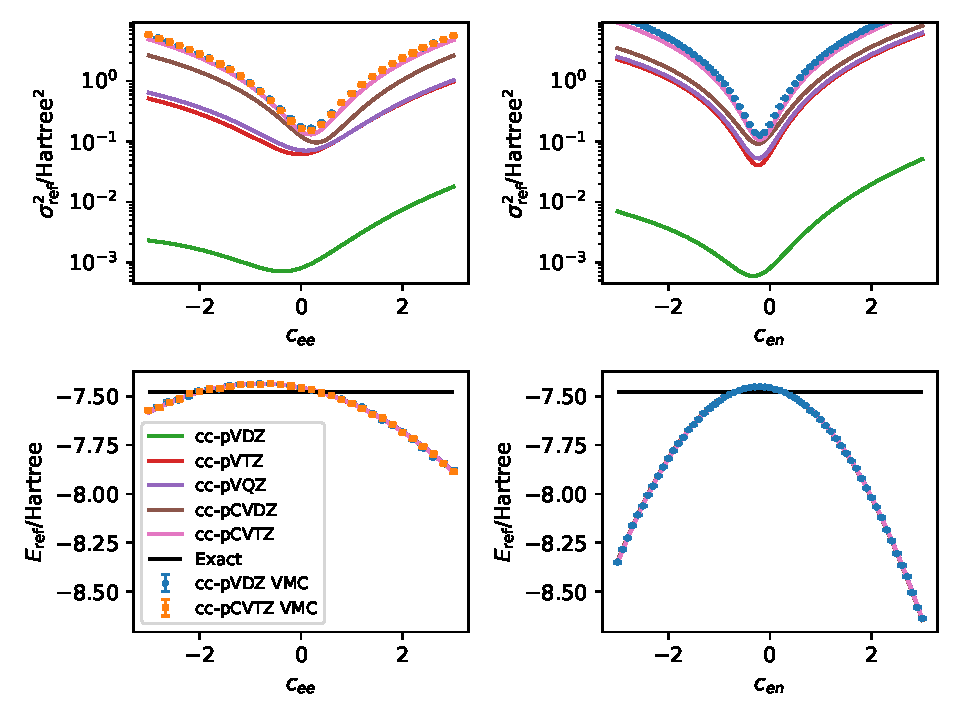
\includegraphics[width=\textwidth]{figures/pytchint/andreea/1parameter}
    \caption{Variance of the reference and reference energy values (top and bottom panels, respectively) with a single-parameter Jastrow factor, for the Li atom with the \vxz{X} basis sets, with $X=$D, T, Q, as well as basis sets core-valence correlation at the double- and triple-zeta level. The left panel introduces an electron-electron term $J_{ee}$ whereas the right panel introduces an electron-nucleus term $J_{en}$. The location of the minimum may be different compared to that obtained by continuum VMC, resulting in a suboptimal Jastrow factor. Data courtesy of Maria-Andreea Filip, who is leading this investigation. Results are preliminary and are intended to be presented in a future publication.}
    \label{fig:det-opt}
\end{figure}

Preliminary results are promising, and this may prove an interesting alternative to \gls{VMC}, or a way of ``correcting'' smaller VMC calculations, to improve efficiency as well as reproducibility.

\section{Parallel Efficiency}

As a benchmark, we calculate N$_2$ with the \avqz basis (14 electrons in 160 orbitals) with the \gls{xTC} approximation. Elapsed time is plotted as a function of the number of compute cores used in figure \ref{fig:parallel-performance}, with favourable scaling. This illustrations the parallel performance of the \pytchint library.

Moreover, thanks to the use of Cython, performance when directly running Fortran when compared to running via Python is roughly identical (468 seconds or 465 seconds with 128 cores for Fortran and Python, respectively).

\begin{figure}[htbp]
    \centering
    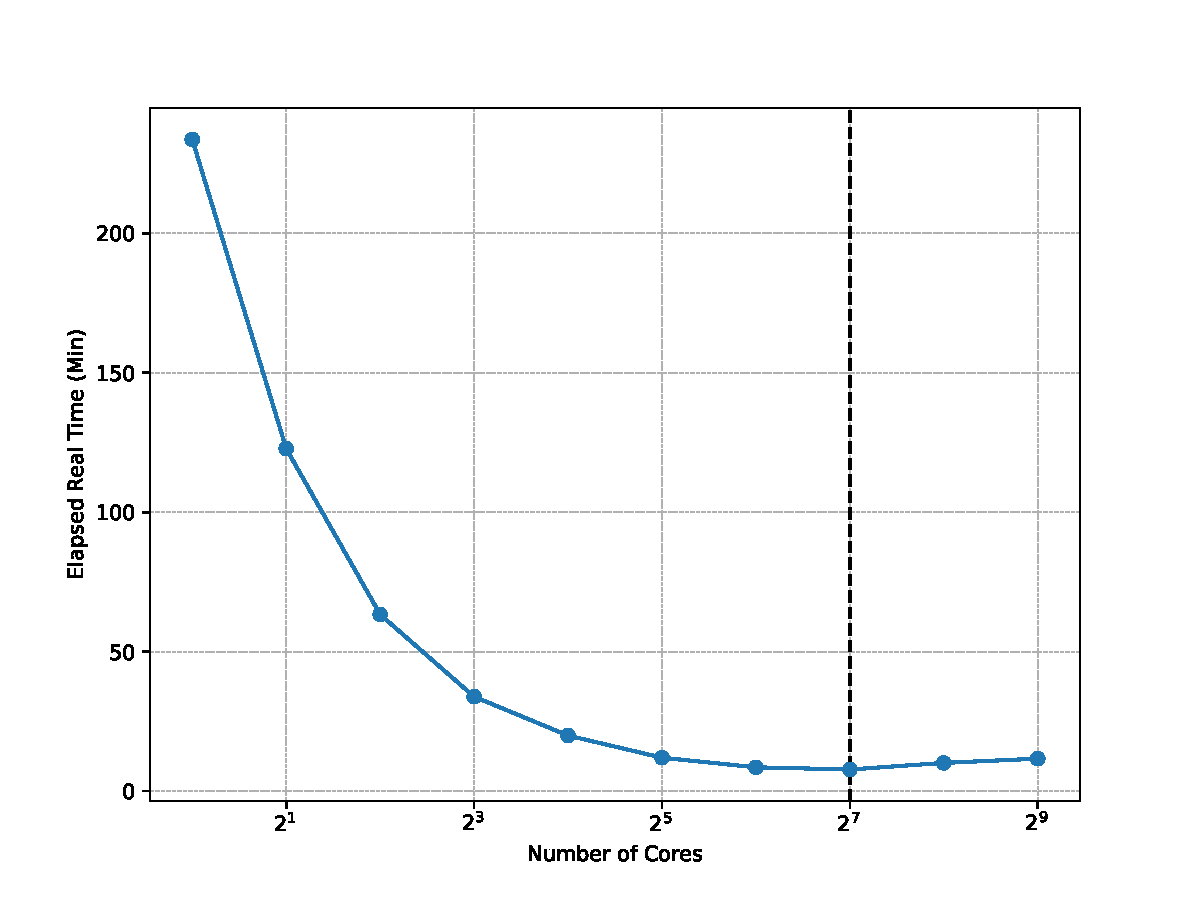
\includegraphics[width=0.8\textwidth]{figures/pytchint/ncore_walltime}
    \caption{Elapsed real time (or walltime) of calculating all-electron transcorrelated integrals under the \gls{xTC} approximation for N$_2$ with the \avqz basis. Note the logarithmic axes. Performance improves drastically when given additional cores, highlighting the parallel capabilities of the \pytchint library. The dotted red line indicates ideal scaling. The dotted vertical line at $2^7$ cores indicates additional nodes. Introducing more nodes, walltime slightly increases, indicating the additional MPI overhead of internode communication is not sufficiently compensated for by the additional cores for this size problem. However, it is worth noting that due to the distributed memory model, these calculations offer similar time performance but the memory load per node is reduced by roughly a factor equal to the number of nodes. Calculations were performed on AMD EPYC 9554 64-Core processors, and each node used 128 cores.}
    \label{fig:parallel-performance}
\end{figure}

\section{Conclusion and Outlook}

Our in-house transcorrelated integral evaluation library is already flexible and performant, and is already used for most TC-related publications from the group. For wider adoption, we plan to improve documentation and ease of use through the Python interface, and have a form of Jastrow optimisation or (quasi-)universal Jastrow form such as those described in \autoref{chap:universal}. This way, \pytchint is a standalone library and would not rely on external software.

Additional features we intend to investigate in the near future are: parallelism with graphics processing units (as our integrals are easily parallelisable), which is already being investigated in the context of TC, further support for periodic solids, and implementing more of the code in high-performance Python to allow easier use of additional features such as automatic differentiation\supercite{wengertSimple1964} with JAX,\supercite{jax2018github} which would allow support for more complex Jastrow factors without the need for manually calculating analytic gradients.
